\documentclass[a4paper,11pt,fleqn]{article}%fleqn pour aligner les equations à gauche
\usepackage{graphicx}
\usepackage[utf8]{inputenc}  
\usepackage[T1]{fontenc}
\usepackage{lscape}

\usepackage{tgheros,textcomp}%Police Arial
\renewcommand{\familydefault}{\sfdefault}

%\setlength{\mathindent}{0pt}%indentation dans math = 0

\usepackage[top = 1cm, bottom = 2cm, left = 1cm, right = 1cm]{geometry}
\usepackage{titlesec}
%\setcounter{secnumdepth}{4}
\usepackage{xcolor}
\usepackage{amssymb} %double flèche de réaction
\usepackage{mathrsfs}%farraday
\usepackage{xtab}%tableau sur plusieurs pages
\usepackage{esvect}%grands vecteurs

\usepackage[version=4]{mhchem} %equations chimiques

\usepackage{array}
\usepackage{chemfig}
\usepackage{multirow}
%\usepackage{sectsty}

\usepackage{caption}
\usepackage{adjustbox}
\usepackage[labelformat=simple]{subfig}
\usepackage{float}


\usepackage{amsmath}
\usepackage{amssymb}
\usepackage[cal=boondoxo]{mathalfa} 
\usepackage{enumitem}
\usepackage{lastpage}
\usepackage{tcolorbox}
\usepackage{siunitx}
\usepackage[european, straightvoltages, RPvoltages]{circuitikz}
\usepackage{tikz}
\usetikzlibrary{shapes.geometric}
\usetikzlibrary{calc}
\usetikzlibrary{automata,positioning}
\usepackage{multicol}
\usepackage{eqnarray}
\usepackage{tabularx,colortbl}%colorer fond cellules

\sisetup{
	detect-all,
	output-decimal-marker={,},
	group-minimum-digits = 3,
	group-separator={~},
	number-unit-separator={~},
	inter-unit-product={~}
} %setup pour SIunitx

\usepackage{listings}%pour insérer le code python
\definecolor{codegreen}{rgb}{0,0.6,0}
\definecolor{codegray}{rgb}{0.5,0.5,0.5}
\definecolor{codepurple}{rgb}{0.58,0,0.82}
\definecolor{backcolour}{rgb}{0.95,0.95,0.92}


%\graphicspath{ {/home/rweye/Documents/Enseignement/2023/Cours/TSPE/Eval/Ressources/} }

\titleformat{\section}
{\titlerule
\vspace{.8ex}%
\normalfont \bfseries}
{\thesection :}{.5em}{\bfseries}

\renewcommand{\thesection}{Exercice \arabic{section}}
\titlespacing{\section}{0pt}{1em}{1em}
\renewcommand{\thesubsection}{\hspace{1cm}\alph{subsection}.}
\renewcommand\thesubfigure{\textbf{Document \arabic{subfigure} :}}

\title{\vspace{-1cm}\large 
	\begin{tabular}{|m{5cm}|>{\centering}m{8cm}|>{\centering\arraybackslash}m{4cm}|}
		\hline
		Nom : & \textbf{\textsc{DS TSPE N°4}} &  Note : \\
		Prénom : & & $\_\_\_$ \textbf{20} \\ \hline
\end{tabular}}
\date{}

\newpagestyle{mystyle}{%
	\setfoot{ROSALIE}{\thepage\,$|$\,\pageref{LastPage}}{}
}
\renewpagestyle{plain}{%
	\setfoot{ROSALIE}{\thepage\,$|$\,\pageref{LastPage}}{}
}

\pagestyle{mystyle}

\newenvironment{itemize*}%
{\begin{itemize}[label=$-$]%
		\setlength{\itemsep}{0pt}%
		\setlength{\parskip}{0pt}}%
	{\end{itemize}}

\newenvironment{itemize**}%
{\begin{itemize}[label=$\_\_$,labelindent=0pt, leftmargin=*,topsep=0pt]%
		\setlength{\itemsep}{0pt}%
		\setlength{\parskip}{0pt}}%
	{\end{itemize}}

\renewcommand{\arraystretch}{1.5}


\begin{document}
\maketitle
\vspace{-2.5cm}
\section{CD et autres supports de l'information}
A partir du début des années 80, le disque audio (CD) a supplanté les vinyles en raison d'une grande facilité d'utilisation et de la quantité d'information stockable. Nous allons, dans un premier temps, étudier un Compact-Disc, puis nous nous intéresserons à la technologie Blue-ray.
\subsection{Le Compact-Disc}
	\begin{enumerate}
		\item Montrer que la surface "utile" $S$ du CD, correspond à la surface grisée du document 1, s'exprime par : $S=\pi \cdot (R_2^2 - R_1^2)$.
		\item On peut estimer la longueur $L$ de la piste par l'expression $L \approx \dfrac{S}{a}$ où $a$ est le pas de la spirale. Évaluer la longueur de la piste de ce CD.
		\item En déduire la durée totale de lecture du CD en minutes.
		\item Lorsque le spot laser se réfléchit autour d'une alvéole, il y a interférences entre la partie de l'onde qui se réfléchit sur le plat et celle qui se réfléchit sur le creux.
		\begin{enumerate}[label=\theenumi.\arabic*]
			\item Proposer un schéma expérimental permettant de mettre en évidence le phénomène d'interférences en décrivant la figure obtenue.
			\item Déterminer la différence de parcours entre l'onde qui se réfléchit sur un creux et celle qui se réfléchit sur un plat.
			\item Ce parcours ayant lieu dans le polycarbonate, déterminer le retard de l'onde réfléchie dans un creux par rapport à l'onde réfléchie sur un plat au niveau du capteur.
			\item Comparer ce retard à la période de l'onde émise par le laser.
			\item En déduire le type d'interférences (constructive ou destructive) entre l'onde réfléchie par un creux et celle réfléchie par un plat au niveau du capteur. La réponse s'appuiera sur un schéma.
			\item Dans ce cas, le signal reçu par le capteur est-il maximal ou minimal ? Commenter. 
		\end{enumerate}
		
		%\item Déterminer la capacité totale théorique d'information (en Mo) que l'on peut enregistrer sur ce CD.
	\end{enumerate}
\subsection{Le Blue-ray}
La technologie Blue-ray a été développée au début des années 2000 afin de commercialiser des films en haute définition. Le principe de fonctionnement est le même que celui d'un CD.
	\begin{enumerate}[resume]
		\item Quelle doit-être la profondeur d'un creux sur un disque Blue-ray ?
		\item Pourquoi ne peut-on pas lire un disque Blue-ray avec un lecteur CD ?
		%\item En supposant que le codage de l'information et la lecture d'un disque Blue-ray sont identiques à ceux d'un CD, déterminer la capacité de stockage qu'aurait un disque Blu-ray. Que peut-on en conclure ?
	\end{enumerate}
\fbox{\begin{minipage}{\textwidth}
	\textbf{Document 1 : Structure d'un CD}\\
	Sur un Compact-Disc, les informations sont stockées sous forme de "creux" et de "plats" le long d'une piste métallique réfléchissante en forme de spirale. Celle-ci commence à une distance $R_1 = \SI{2,5}{cm}$ de l'axe du CD et se termine à une distance $R_2 = \SI{6,0}{cm}$.\\
	La portion grisée correspond à la partie du CD occupée par la piste métallique. Un extrait de la piste est représenté à coté. Le pas de la spirale est $a = \SI{1,6}{\micro\meter}$.\\
	Lors de la rotation du disque, les structures porteuses de l'information défilent devant un système optique à la vitesse linéaire constante $V=\SI{1,2}{\meter\per\second}$.
	\begin{center}
	
\includegraphics[width=\textwidth]{Ressources/TSPE_DS4_Fig1.png}
	\end{center}
\end{minipage}}

\noindent \fbox{\begin{minipage}{\textwidth}
	\textbf{Document 2 : Principe optique de lecture d'un CD}\\
	La piste physique est constituée d'alvéoles d'une largeur de \SI{0,67}{\micro\meter}, d'une profondeur $h_c = \SI{0,12}{\micro\meter}$ et de longueur variable. On nomme "creux" le fond  d'une alvéole et "plat" l'espace entre deux alvéoles.
	\begin{center}
	
\includegraphics[width=.5\textwidth]{Ressources/TSPE_DS4_Fig2.png}
	\end{center}
	La tête de lecture est composée d'un laser émettant un faisceau lumineux et d'une cellule photoélectrique chargée de capter le faisceau réfléchi. Le laser utilisé pour lire les CD a une longueur d'onde $\lambda_0 =\SI{780}{nm}$ dans l'air et $\lambda = \SI{503}{nm}$ dans le polycarbonate.\\
	La profondeur $h_c$ des creux est liée à la longueur d'onde $\lambda$ du laser dans le polycarbonate par la relation : $2\cdot h_c = \dfrac{\lambda}{2}$\\
	La vitesse de propagation de la lumière émise par le laser dans le polycarbonate vaut $\SI{1,93E8}{\meter\per\second}$.
\end{minipage}}

\noindent \fbox{\begin{minipage}{\textwidth}
	\textbf{Document 3 : Comparaison entre CD, DVD et Blu-ray}\\
	\begin{center}
	
\includegraphics[width=.8\textwidth]{Ressources/TSPE_DS4_Fig3.png}
	\end{center}
	\begin{tabular}{|>{\centering}m{3cm}|>{\centering}m{4cm}|>{\centering}m{4cm}|>{\centering\arraybackslash}m{4cm}|} \hline
	\textbf{Type de support} & CD & DVD & Blu-ray\\ \hline
	\textbf{Longueur d'onde dans l'air} & \SI{780}{nm} & \SI{650}{nm} & \SI{405}{nm}\\ \hline
	\textbf{Longueur d'onde dans le polycarbonate} & \SI{503}{nm} & \SI{419}{nm} & \SI{261}{nm}\\ \hline
	\textbf{Capacité réelle de stockage} & \SI{700}{Mo}& \SI{4,7}{Go}& \SI{25}{Go}\\ \hline
	\textbf{Distances entre les pistes} & \SI{1,6}{\micro\meter}& \SI{0,74}{\micro\meter}& \SI{0,3}{\micro\meter}\\ \hline
	\textbf{Largeur du faisceau} & \SI{2,1}{\micro\meter}& \SI{1,2}{\micro\meter}& \SI{0,6}{\micro\meter} \\ \hline
	\textbf{Longueur de la piste} & & \SI{11,7}{km} & \SI{27}{km}\\ \hline
	\end{tabular}
\end{minipage}}

\section{Réalisation d'une pile nickel-zinc}
On réalise une pile formée à partir des couples \ce{Ni^2+}/\ce{Ni} et \ce{Zn^2+}/\ce{Zn}. Chaque solution a pour volume $V = \SI{100}{mL}$ et la concentration initiale des ions positifs est $C = \SI{5,0E-2}{\mole\per\liter}$.\\
\textbf{Données :}
\begin{itemize}
	\item \textbf{Masse molaire du zinc :} $M(\ce{Zn}) = \SI{65,4}{\gram\per\mole}$
	\item \textbf{Masse molaire du nickel :} $M(\ce{Ni}) = \SI{58,7}{\gram\per\mole}$
	\item \textbf{Charge élémentaire de l'électron :} $e= \SI{-1,6E-19}{C}$
	\item \textbf{Constante d'Avogadro :} $N_A = \SI{6,02E23}{\per\mole}$
	\item \textbf{Constante de Faraday :} $F = \SI{9,65E4}{C}$
	\item Pour la réaction suivante : \ce{Ni^2+ + Zn = Zn^2+ + Ni}, la constante d'équilibre vaut $K = 10^{18}$.
\end{itemize}
\newpage
\begin{enumerate}
	\item \textbf{Réalisation de la pile}
	\begin{enumerate}[label=\theenumi.\arabic*]
		\item L'électrode positive de cette pile est l'électrode de nickel. Légender le schéma de la \textbf{Figure 1} en annexe avec les termes suivants : électrode de nickel, électrode de zinc, pont salin, solution contenant des ions \ce{Zn^2+}, solution contenant des ions \ce{Ni^2+}.
		\item Écrire les demi-équations des réactions se produisant aux électrodes. Préciser à chaque électrode s'il s'agit d'une oxydation ou d'une réduction.
		\item Écrire l'équation de la réaction globale qui intervient quand la pile débite.
		\item Calculer la valeur du quotient réactionnel initial $Q_{r,i}$. Cette valeur est elle cohérente avec la polarité proposée ?
	\end{enumerate}
	\item \textbf{Étude de la pile}
	\begin{enumerate}[label=\theenumi.\arabic*]
		\item On fait débiter la pile dans un conducteur ohmique. Compléter le schéma de la \textbf{Figure 1}
		\item Préciser sur ce schéma le sens du courant et le sens de déplacement des électrons dans le circuit extérieur.
		\item Comment varie la concentration des ions positifs dans chacun des béchers ? En déduire l'évolution du quotient de réaction $Q_r$.
		\item Sachant que la masse des électrodes ne limite pas la réaction, pour quelle raison la pile s'arrêtera-t-elle de débiter ? Quelle est alors la valeur de $Q_r$ ?
		\item La réaction étant considérée totale, calculer l'avancement maximal $x_{max}$ de la réaction.
		\item Quelle relation existe-t-il entre $x_{max}$ et la quantité de matière d'électrons qui ont circulé ?
		\item En déduire la charge totale de la pile.
	\end{enumerate}
\end{enumerate}

\vspace{2cm}
\begin{figure}[h!]
    \centering
    \caption*{\textbf{Figure 1}}
    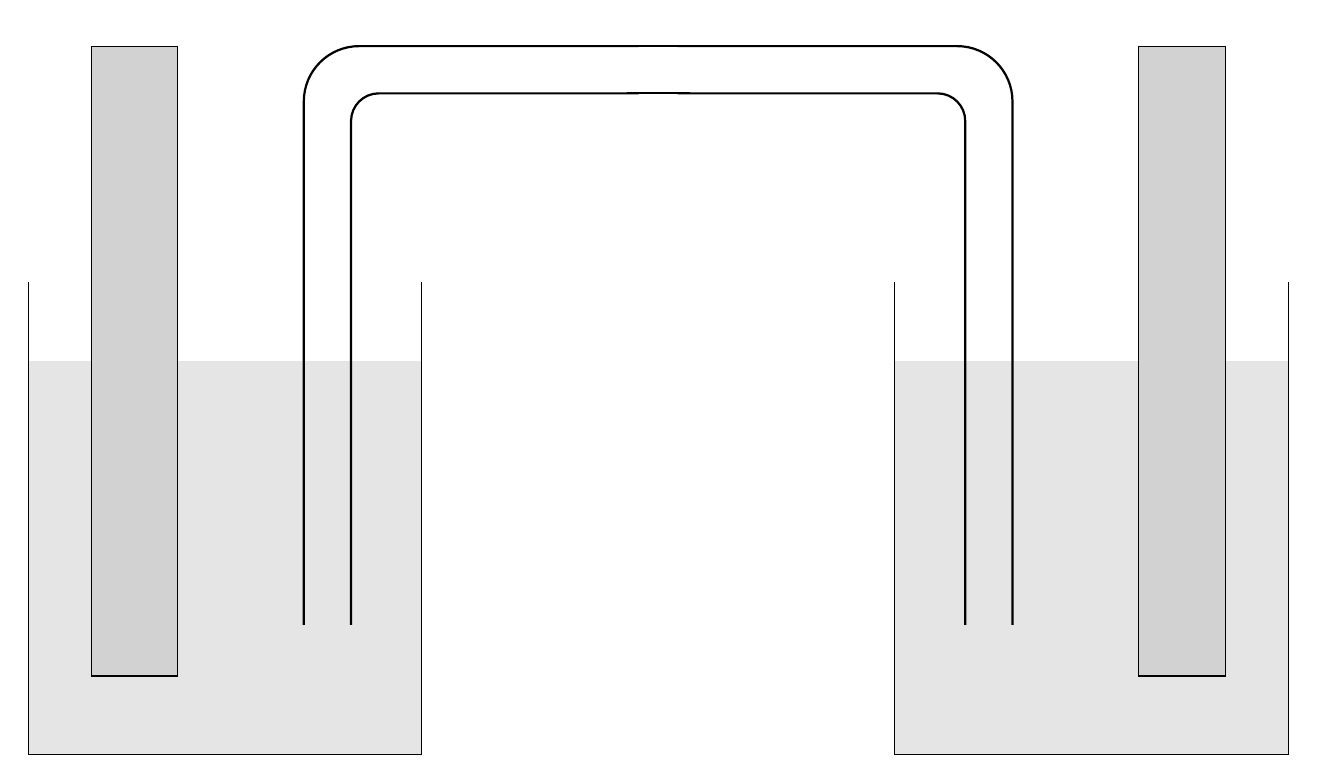
\begin{tikzpicture}[scale=2,transform shape]
    %%%%%%%%%%%%%%%%%%%%%%%%%%%%%%%%%%%%%% Béchers
    \fill[gray!20] (-1.5,0)--(-4,0)--(-4,2.5)--(-1.5,2.5)--cycle;
    \fill[gray!20] (1.5,0)--(4,0)--(4,2.5)--(1.5,2.5)--cycle;
    
    \draw (-1.5,0)--(-1.5,3);
    \draw (-1.5,0)--(-4,0);
    \draw (-4,0)--(-4,3);

    \draw (1.5,0)--(1.5,3);
    \draw (1.5,0)--(4,0);
    \draw (4,0)--(4,3);

    %%%%%%%%%%%%%%%%%%%%%%%%%%%%%%%%%%%%%% Plaques
    \filldraw[gray!35,draw=black] (-3.05,0.5)--(-3.6,0.5)--(-3.6,4.5)--(-3.05,4.5)--cycle;
    \filldraw[gray!35,draw=black] (3.05,0.5)--(3.6,0.5)--(3.6,4.5)--(3.05,4.5)--cycle;
    
    %%%%%%%%%%%%%%%%%%%%%%%%%%%%%%%%%%%%%% Pont salin
    \tikzstyle{suite}=[-,thick,rounded corners=10pt]
    \node (b1) at (1.95,0.7){};
    \node (a1) at (-1.95,0.7){};
    \node (i1) at (0,4.2){};

    \draw[suite] (b1)|-(i1)-|(a1.north) ;
    
    \node (b2) at (2.25,0.7){};
    \node (a2) at (-2.25,0.7){};
    \node (i2) at (0,4.5){};
    \tikzstyle{suite2}=[-,thick,rounded corners=20pt]
    \draw[suite2] (b2)|-(i2)-|(a2.north) ;
    \draw[thick] (-0.2,4.2) -- (0.2,4.2);
    \draw[thick] (-0.2,4.5) -- (0.2,4.5);
\end{tikzpicture}
\end{figure}

\end{document}